\documentclass[hidelinks,12pt]{article}

\usepackage{setspace}
\usepackage{lipsum}
\usepackage{geometry} % Optional: For better control of page margins

\usepackage{amssymb,amsmath,amsfonts,float,eurosym,geometry,ulem,graphicx,color,setspace,sectsty,comment,natbib,pdflscape,subfigure,array,booktabs}

\usepackage[absolute,overlay]{textpos} % Allows absolute positioning
\usepackage[bottom]{footmisc}
\usepackage{afterpage}

\usepackage{hyperref,cleveref}
\hypersetup{
    colorlinks=true,
    linkcolor=blue,
    filecolor=blue,      
    urlcolor=blue,
    citecolor=blue,
    pdftitle={Overleaf Example},
    pdfpagemode=FullScreen,
    }
\urlstyle{same}

\usepackage{graphicx}
\usepackage{ragged2e}
\usepackage{adjustbox}
\usepackage{booktabs}
\usepackage{dcolumn}

\usepackage[style=apa, sorting=nyt]{biblatex}
\addbibresource{cite.bib}

\usepackage{booktabs}
\usepackage[flushleft]{threeparttable}

\usepackage[flushleft]{caption}
\newcommand\fnote[1]{\captionsetup{font=footnotesize}\caption*{#1}}

\usepackage[skip=10pt plus1pt, indent=0pt]{parskip}
\usepackage[capposition=top]{floatrow}

\newcommand{\tabnotes}[2]{\bottomrule \multicolumn{#1}{@{}p{0.70\linewidth}@{}}{\footnotesize #2 }\end{tabular}\end{table}}

\usepackage [english]{babel}
\usepackage [autostyle, english = american]{csquotes}
\MakeOuterQuote{"}

\normalem

\onehalfspacing
\newtheorem{theorem}{Theorem}
\newtheorem{corollary}[theorem]{Corollary}
\newtheorem{proposition}{Proposition}
\newenvironment{proof}[1][Proof]{\noindent\textbf{#1.} }{\ \rule{0.5em}{0.5em}}

\newtheorem{hyp}{Hypothesis}
\newtheorem{subhyp}{Hypothesis}[hyp]
\renewcommand{\thesubhyp}{\thehyp\alph{subhyp}}

\newcommand{\red}[1]{{\color{red} #1}}
\newcommand{\blue}[1]{{\color{blue} #1}}

\newcolumntype{L}[1]{>{\raggedright\let\newline\\arraybackslash\hspace{0pt}}m{#1}}
\newcolumntype{C}[1]{>{\centering\let\newline\\arraybackslash\hspace{0pt}}m{#1}}
\newcolumntype{R}[1]{>{\raggedleft\let\newline\\arraybackslash\hspace{0pt}}m{#1}}

\renewcommand{\arraystretch}{1.3}

\geometry{left=1.0in,right=1.0in,top=1.0in,bottom=1.0in}

%%% for flowcharts
\usepackage{tikz}
\usetikzlibrary{shapes.geometric, arrows}
\tikzstyle{startstop} = [rectangle, rounded corners, text width=8.5cm, minimum width=3cm, minimum height=1cm,text centered, draw=black, fill=white]
\tikzstyle{notes} = [rectangle, rounded corners, text width=4cm, minimum height=1cm, align=right, fill=white]
\tikzstyle{process} = [rectangle, rounded corners, text width=4cm,  minimum height=1cm, text centered, draw=black, fill=white]
\tikzstyle{decision} = [diamond, text width=2.5cm, text centered, draw=black, fill=white]
\tikzstyle{arrow} = [thick,->,>=stealth]

\begin{document}


\begin{singlespace}

\begin{titlepage}
\title{Bureaucrats' Stated vs. Revealed Policy Preferences: Evidence from Teachers' Responses to an Education Reform in Tanzania}
%\title{Do Policies Shift Bureaucrat Beliefs? Evidence from Education Reforms and a Teacher Experiment}

\author{Frank Odhiambo \thanks{Development Economics, University of G\"ottingen, Germany. E-mail: \href{mailto:frank.odhiambo@wiwi.uni-goettingen.de}{frank.odhiambo@wiwi.uni-goettingen.de}.}}

\date{\today}
\maketitle
\begin{abstract}
\begin{singlespace}
Policy reforms succeed only when bureaucrats implement them effectively, but implementation may depend on whether bureaucrats actually support the policies. This paper investigates frontline bureaucrats’ responses, both stated and revealed, to top-down policy reforms. Drawing on evidence from Tanzania’s nationwide free primary education (FPE) reform, and using a difference-in-differences design, I find that teachers' stated preference for FPE increases by 18 percentage points post-reform. Yet this increase in stated preference coincides with an adverse behavioral response: rent-seeking. Over 34\% of eligible parents report paying a bribe to secure school placement for their child, and public perceptions of teacher corruption rise by 32 percentage points. These results suggest that frontline bureaucrats can simultaneously endorse a policy in principle while undermining its implementation in practice, challenging the conventional assumption that stated support guarantees fidelity. The findings highlight the need to consider bureaucratic incentives beyond attitudinal alignment when designing large-scale reforms. More broadly, the study contributes to understanding the interplay between bureaucrat attitudes and their behavioral responses to policy reforms, particularly in developing-country contexts.\\
\end{singlespace}

\textbf{Keywords:} Policy implementation, bureaucratic behavior, education reform, corruption, Tanzania \\

JEL Classification: H11, I21, D73, O15

\bigskip
\end{abstract}
\setcounter{page}{0}
\thispagestyle{empty}
\end{titlepage}
\pagebreak \newpage

\onehalfspacing

\section{Introduction}
\hspace{1em} The implementation success of many reforms often depends on the actions of frontline bureaucrats who translate policy directives into practice. While policymakers design reforms with specific objectives, the ultimate success of these interventions depend on whether implementing agents adopt behaviors consistent with policy goals. This paper examines this implementation challenge in the context of a nationwide reform that eliminated primary school fees in Tanzania. I examine how teachers as the key bureaucratic actors in schools responded to the reform, both in stated support and behaviorally.

I build on standard principal-agent models where policymakers (principals) design reforms that must be implemented by bureaucrats (agents) operating under different constraints and incentives. Policymakers, such as legislators and senior government officials, prioritize broad policy objectives, whereas bureaucrats operate under local constraints and hold discretion over day-to-day implementation. In education, teachers and school administrators embody the agent role, exercising influence that can either advance or undermine policy goals depending on how their beliefs and incentives align with those of the principal.

Existing research establishes that bureaucrat beliefs significantly influence implementation outcomes. For example, in educational settings, teachers' attitudes and expectations affect student achievement and educational choices (\cite{sabarwal_teacher_2022,fives_teachers_2016,liou_climate_2021}) with particularly strong evidence on how gender stereotypes shape course selection and long-term human capital formation (\cite{lavy_gender_2008,lavy_origins_2018}). More broadly, studies from various institutional contexts demonstrate that pre-existing norms and enforcement capacity determine compliance behavior. For instance, \textcite{fisman_corruption_2007} show how cultural norms affected diplomatic parking violations and \textcite{olken_monitoring_2007} documents how monitoring intensity reduces corruption in Indonesian infrastructure projects. These studies suggest that attitudes are important for implementation fidelity, but that incentives and constraints may also determine whether attitudes translate into compliant behavior.

More recently, economists have examined how policy actors update beliefs in response to new information. \textcite{vivalt_how_2023} show that policymakers and bureaucrats hold systematically different priors and that new evidence can shift those priors, with heterogeneous responsiveness. In related work from Brazil, \textcite{hjort_how_2021} demonstrate that mayors revise beliefs about early childhood programs when presented with credible evidence, although the pattern of updating differs from \textcite{vivalt_how_2023}. This literature establishes that beliefs are malleable and policy-relevant. Less is known, however, about whether and how a concrete top-down reform shifts implementers’ beliefs and their on-the-ground behaviors, and whether those two margins move in tandem or come apart.

This paper contributes to three strands of the literature. First, it advances research on belief updating in bureaucratic settings by moving beyond informational treatments to study responses to an actual reform mandate. Whereas most work examines whether new information shifts stated attitudes, I show how posterior beliefs translate---or fail to translate---into implementation. Second, the paper links the literature on stated versus revealed preferences to the domain of public sector behavior. By distinguishing between expressed support and observed implementation, the framework demonstrates that belief change may manifest as surface-level compliance unless institutional constraints align incentives with reform objectives. Third, the analysis contributes to the study of policy implementation in low-capacity states. It highlights how weak monitoring and rent-seeking opportunities generate divergence between policy intentions and outcomes, even when attitudes shift in the direction of the principal. 

Empirically, I assemble nationally representative survey data spanning periods before and after the FPE reform and combine them with measures of teachers’ policy attitudes and multiple indicators of behavior relevant to implementation. To identify reform effects, I employ a difference-in-differences design that exploits temporal variation around the policy coupled with cross-sectional comparisons to appropriate counterfactual groups. For attitudes, I compare changes for teachers relative to other groups not directly charged with school-level implementation. For behavior, I study household interaction with schools, specifically, whether eligible parents report paying a bribe to secure a child’s place. I also benchmark teacher's perception-based corruption measures against other occupational groups. 

My main results highlight a disconnect between teachers’ stated support for FPE and their behavioural response. Teachers’ support for FPE rises by 18 percentage points following the reform. Yet, this postive attitudinal shift coincides with increased rent-seeking behavior: about 34\% of eligible parents report paying a bribe for school placement and public reports of teacher corruption increase by 32 percentage points. This pattern suggests a "stated preference-revealed preference" divergence such as those discussed by \textcite{beshears_how_2008}. In this setting, implementers endorse reform objectives while simultaneously engaging in behaviors that undermine equitable access.

The evidence points to a demand-side mechanism: the reform generated a surge in enrollment demand that, combined with capacity constraints, increased teachers' discretionary power over scarce school slots. This enhanced gatekeeping authority created opportunities for rent extraction despite teachers' stated support for the policy's egalitarian goals.

These findings have important implications for reform design and implementation. Stated bureaucratic support, while potentially necessary, is insufficient for ensuring implementation fidelity. Policymakers must anticipate how large-scale interventions reshape local incentives and alter the distribution of discretionary authority, particularly in weak monitoring environments. Reforms intended to expand access may inadvertently create barriers for intended beneficiaries if implementation challenges are not adequately addressed.

The remainder of the paper proceeds as follows. Section 2 describes the Tanzanian education context and FPE reform. Section 3 presents the data and empirical methodology. Section 4 reports results on attitude and behavior changes, including robustness checks and heterogeneity analysis. Section 5 discusses mechanisms and policy implications. Section 6 concludes.

%\section{Tanzania's universal education reform}
%TBD


\section{Theoretical framework}\label{sec:theory}

In the principal--agent framework, the free primary education (FPE) reform represents a directive from the principal (the state) that teachers, as agents, are expected to implement. The agent’s response to the reform can be separated into two distinct but interrelated domains: the expression of stated preferences and the choice of behavioral implementation. Distinguishing between these two domains is critical, as information shocks may shift stated support without necessarily translating into behavioral compliance.

Let an agent $i$ hold prior beliefs $B_{0i}\in\{\text{Support},\text{Oppose}\}$ about the effectiveness of FPE. Upon announcement of the reform, the agent receives a signal $T_i$, which may induce belief updating. Define $U_i\in\{0,1\}$ as an indicator of belief updating, where $U_i=1$ if posterior beliefs $B_i$ differ from $B_{0i}$. Agents then express a stated preference $S_i\in\{0,1\}$, with $S_i=1$ denoting expressed support. Stated preferences, however, may not perfectly reveal posterior beliefs: social desirability, reputational concerns, or alignment with institutional norms may induce agents to declare support even if privately unconvinced.

The decisive outcome for policy success is the agent’s implementation choice $I_i\in\{0,1\}$, where $I_i=1$ if the teacher complies with the reform (e.g.\ eliminating school fees). In a setting without outside incentives or costs, implementation would follow directly from posterior beliefs: $B_i=\text{Support}$ implies $I_i=1$, while $B_i=\text{Oppose}$ implies $I_i=0$. In practice, however, weak monitoring ($M_i$) and the presence of alternative rent-extraction opportunities ($R_i$) allow for strategic compliance: agents may publicly declare support ($S_i=1$) while simultaneously engaging in partial or non-compliance ($I_i=0$). This wedge between stated preferences and revealed behavior creates implementation risk, as policy outcomes become contingent not only on belief dynamics, but also on incentive compatibility.

Aggregate implementation is therefore given by:
\begin{equation} 
\theta = \mathbb{E}[I_i] = \pi_0 (1-\alpha) + (1-\pi_0)\alpha\rho + \pi_0 \alpha(1-\rho)
\end{equation} 

where $\pi_0$ is the share of initial supporters, $\alpha = \Pr(U_i=1)$ is the probability of updating, and $\rho$ is the probability that updating leads to support. Policy success requires $\theta \geq \theta^*$, a threshold level of compliance. In the absence of monitoring and with high rents, $\theta$ may fall short of $\theta^*$ even when $\rho$ is large, reflecting a regime of surface-level compliance where belief updating affects $S_i$ but not $I_i$.

\section{Methods and Data}
I test my theoretical model using two main approaches. First, I test, quasi-experimentally whether agents do in fact update beliefs, and subsequently, their compliance. Second, to test the mechanisms discussed in my estimation, I run a experiment in which I directly assign an exogenous signal, document prior beliefs, test whether posterior beliefs are updated, and whether that leads to implementation compliance. I discuss both in more detail below.

\subsection{DiD Analysis}\label{sec:econometrics}
Because the FPE reform under discussion was universal, to identify the effects of FPE reforms on both teachers’ beliefs and eventual behavioral responses, I estimate difference-in-differences (DiD) models. The first specification examines whether teachers update their stated support of the policy $S_i$, while the second investigates whether teachers engage in rent-seeking behavior following the reform, a proxy for changes in ($I_i=0$). Together, these estimates should reveal whether any changes in the stated support reflect only surface-level compliance. A positive $\beta_{DiD}$ in the support specification (Equation~\ref{eq:beliefs}) combined with a null or negative $\kappa_{DiD}$ in the rent-seeking specification (Equation~\ref{eq:rentseeking}) represents behavioral outcomes consistent with surface-level compliance.

\subsubsection{Stated support for the policy}
To estimate teachers’ stated beliefs before and after the reform to those of a control group (e.g.\ other educated adults) I estimate following model:  
\vspace{-1em}

\begin{equation} 
S_{itd} = \beta_0 + \beta_1 \text{Teacher}_i + \beta_2 \text{Post}_t + \beta_{DiD} (\text{Teacher}_i \times \text{Post}_t) + X_{it}\gamma + \mu_{d} + \varepsilon_{itd}
\label{eq:beliefs}
\end{equation}
where $S_{it}$ represents stated support for the reform, $\text{Teacher}_i$ is an indicator for teachers, $\text{Post}_t$ marks the post-policy period and $\mathbf{X}_{i}$ is a vector of individual-level controls (age and education). District fixed effects $\mu_{d}$ absorb time-invariant unobserved heterogeneity, and standard errors are clustered at the district level. The coefficient of interest is $\beta_{DiD}$, which captures the differential change in support for FPE among teachers relative to non-teachers after the reform.

\subsubsection{Rent-seeking}
As mentioned previously, rent-seeking by teachers signals (partial) non-compliance with the policy. To investigate this, I estimate an analogous model that captures changes in survey participants perception of teacher corruption, relative to other public servants corruption. Using other public servants' reported corruption (for example, police officers, judges etc) as a counterfactual helps to absorb general corruption trends within the country. Observing the public's reports of teacher rent-seeking, is a more reliable measure than, say, teachers' self reported rent-seeking responses due to social desirability concerns. I implement the following specification:  
\vspace{-1.5em}

\begin{equation} \label{eq:rentseeking}
    I_{itd} = \alpha + \theta_1 \, \text{Teacher}_{i} 
    + \theta_2 \, \text{Post}_{t} 
    + \kappa_{DiD} \, (\text{Teacher}_{i} \times \text{Post}_{t})
    + \mathbf{X}_{i}' \lambda 
    + \mu_{d} + \varepsilon_{itd},
\end{equation}
where $I_{it}$ represents a corruption report for individual $i$ in district $d$ at time $t$, a proxy for non-compliance, $\text{Teacher}_{i}$ is a binary representing whether the corruption report relates to a teacher and 0 if other public servant. All other variables are defined as above. The coefficient of interest $\kappa_{DiD}$ measures the extent to which reports of teacher corruption changes in the post-reform period relative to the pre-reform period, relative to other public servants.

\subsubsection{Data}
I use nationally representative survey data from the Afrobarometer project for Tanzania. Specifically, I draw on Rounds 1--3 of the survey, which were implemented in 2001, 2003, and 2005, respectively. The Afrobarometer is a repeated cross-sectional survey designed to capture citizen attitudes, experiences, and evaluations of democracy, governance, and service delivery across African countries. In Tanzania, the sampling strategy follows a stratified, clustered and nationally representative design, allowing inference at the population level.  

The period covered by these data is particularly well suited to study the effects of Tanzania's free primary education (FPE) reform on teacher beliefs and behaviors. While the policy was announced in 2001, it was officially implemented in 2002. This means that Round 1 provides a baseline measure of beliefs and behaviors just prior to implementation, while Rounds 2 and 3 capture responses in the immediate aftermath of the reform. 

\subsection{Experimental validation}  
To directly test the mechanisms, I consider a complementary experiment in which teachers are randomly assigned to receive exogenous policy signals. The reduced-form models are
\begin{align}
S_i &= \alpha_0 + \alpha_1 T_i + \alpha_2 X_i + \eta_i, \label{eq:stated}\\
I_i &= \delta_0 + \delta_1 T_i + \delta_2 X_i + \nu_i, \label{eq:behavior}
\end{align}
where $T_i$ is the randomized policy signal, and $X_i$ is a vector of teacher and school covariates. A finding that $\alpha_1\neq 0$ while $\delta_1=0$ would indicate that information shifts stated support without translating into behavioral compliance, consistent with surface-level compliance.

To estimate the causal effect of belief updating on implementation, $T_i$ can be used as an instrument for posterior beliefs or the updating indicator $U_i$. The corresponding two-stage least squares (2SLS) specification is
\begin{align}
U_i &= \pi_0 + \pi_1 T_i + \pi_2 X_i + \varepsilon_i, \label{eq:first-stage}\\
I_i &= \gamma_0 + \gamma_1 \widehat{U}_i + \gamma_2 X_i + \xi_i, \label{eq:second-stage}
\end{align}
where $\widehat{U}_i$ is the fitted value from the first stage. The coefficient $\gamma_1$ identifies the local average treatment effect of belief updating on implementation for compliers.

Finally, to capture the moderating role of institutional enforcement, the implementation equation can be extended to include monitoring $M_i$:
\begin{equation}
I_i = \zeta_0 + \zeta_1 U_i + \zeta_2 M_i + \zeta_3 (U_i \times M_i) + \kappa' X_i + \varepsilon_i.
\label{eq:monitoring}
\end{equation}
In this specification, $\zeta_1$ measures the baseline effect of belief updating on compliance, while $\zeta_3$ tests whether stronger monitoring amplifies the translation of updated beliefs into behavioral compliance. Evidence of $\zeta_1=0$ but $\zeta_3>0$ would support the hypothesis that belief updating produces only surface-level compliance.

This framework generates three  important predictions. First, if information primarily affects attitudes without changing incentives, we expect $\alpha_1>0$ in equation~\eqref{eq:stated} but $\delta_1=0$ in equation~\eqref{eq:behavior}, indicating with surface-level compliance. Second, if belief updating causally shapes behavior, the instrumental variable estimate $\gamma_1$ in equation~\eqref{eq:second-stage} should be strictly positive. Third, the effect of belief updating on implementation should be heterogeneous with respect to monitoring: $\zeta_3>0$ in equation~\eqref{eq:monitoring} implies that enforcement strengthens the translation of beliefs into action. Observing these interaction patterns would support the interpretation that stated preferences and implementation diverge when incentives are misaligned, highlighting the central role of enforcement in translating belief change into effective policy execution.

%In sum, information treatments can shift stated preferences without necessarily altering implementation behavior, and the translation of beliefs into action depends on monitoring and rent-extraction opportunities. The DiD design exploits the universal reform to document these patterns at scale, while the experiment provides a micro-founded test of the mechanisms. Together, these approaches allow me to assess not only whether beliefs update in response to the reform, but also whether such updating meaningfully affects bureaucratic behavior or remains at the level of surface compliance.

%\section{Background characteristics}

%TBD

\section{Results}

\subsection{Stated support for policy}
In Table \ref{did_beliefs_main}, presents estimates of the effect of Tanzania’s Free Primary Education (FPE) reform on teachers’ stated beliefs. We observe some key results. Prior to the reform, teachers’ beliefs are not systematically different from those of the general population. Following the reform, both teachers and the general populations' stated preferences for free primary education shifted in the direction of the policy, even though teachers updated their preferences more, by about 18 percentage points. However, we also observe that more educated respondents, those with secondary or tertiary level schooling, were likely to express beliefs consistent with the reform compared to those with primary or less schooling.


\begingroup
\setlength{\tabcolsep}{14pt}  % Increase space between columns
\begin{table}[H]
   \begin{singlespace}
    \centering
    \fontsize{11pt}{10pt}\selectfont  % Sets the font size locally inside the table
    \caption{Teachers' stated beliefs post-reform} \label{did_beliefs_main}
    \resizebox{0.85\textwidth}{!}{%
    \begin{threeparttable}
        
\begin{tabular}{l D{.}{.}{4.6} D{.}{.}{4.6} D{.}{.}{4.6}}
\toprule
 & \multicolumn{1}{c}{1} & \multicolumn{1}{c}{2} & \multicolumn{1}{c}{3} \\
\midrule
Teacher x Post        & 0.187^{**}              & 0.172^{*}               & 0.180^{**}              \\
                      & (0.090)                 & (0.088)                 & (0.089)                 \\
Teacher               & -0.068^{*}              & 0.047                   & 0.015                   \\
                      & (0.037)                 & (0.037)                 & (0.038)                 \\
Post                  & 0.416^{***}             & 0.402^{***}             & 0.405^{***}             \\
                      & (0.026)                 & (0.022)                 & (0.026)                 \\
Age                   &                         & 0.000^{*}               & 0.000^{*}               \\
                      &                         & (0.000)                 & (0.000)                 \\
Secondary education   &                         & -0.124^{***}            & -0.117^{***}            \\
                      &                         & (0.020)                 & (0.019)                 \\
Tertiary education    &                         & -0.190^{***}            & -0.157^{***}            \\
                      &                         & (0.024)                 & (0.024)                 \\
\midrule
District FE           & \multicolumn{1}{c}{Yes} & \multicolumn{1}{c}{No}  & \multicolumn{1}{c}{Yes} \\
Controls              & \multicolumn{1}{c}{No}  & \multicolumn{1}{c}{Yes} & \multicolumn{1}{c}{Yes} \\
Num. obs.             & 3443                    & 3432                    & 3432                    \\
Num. groups: district & 129                     &                         & 129                     \\
\bottomrule
\end{tabular}

        \begin{tablenotes}
            %\vspace{-2mm} % Adjust spacing as needed
             \small % Adjust font size as needed
            \textbf{Notes}: Table shows changes in teachers' stated beliefs post Tanzania's FPE reform. Cluster-robust standard errors in parenthesis with the following significance levels: {$^{*}$p$<$0.1; $^{**}$p$<$0.05; $^{***}$p$<$0.01}.
        \end{tablenotes}
    \end{threeparttable}}
    \end{singlespace}
\end{table}
\endgroup

\subsection{Behavioral responses}
Table \ref{did_rent_main} presents difference-in-differences estimates of changes in perceived teacher corruption relative to other public officials. Although teachers were viewed as less corrupt at baseline, the reform led to a relative increase in their perceived corruption, particularly when compared to police and elected leaders. This shift occurred despite an overall decline in perceived corruption across officials, indicating that teachers’ reputational advantage diminished and pointing to rent-seeking behavior through bribery.

\begingroup
\setlength{\tabcolsep}{18pt}  % Increase space between columns
\begin{table}[h]
   \begin{singlespace}
    \centering
    \fontsize{11pt}{10pt}\selectfont  % Sets the font size locally inside the table
    \caption{Changes in perceptions about teacher corruption relative to...} \label{did_rent_main}
    \resizebox{0.85\textwidth}{!}{%
    \begin{threeparttable}
        
\begin{tabular}{l c c c}
\toprule
 & Police & Judge & Elected leader \\
\midrule
Teacher               & $-0.656^{***}$ & $-0.381^{***}$ & $-0.309^{***}$ \\
                      & $(0.012)$      & $(0.020)$      & $(0.018)$      \\
Post                  & $-0.398^{***}$ & $-0.207^{***}$ & $-0.340^{***}$ \\
                      & $(0.015)$      & $(0.027)$      & $(0.028)$      \\
Age                   & $-0.000$       & $-0.000$       & $-0.000$       \\
                      & $(0.000)$      & $(0.000)$      & $(0.000)$      \\
Secondary education   & $0.065^{***}$  & $0.054^{***}$  & $0.073^{***}$  \\
                      & $(0.013)$      & $(0.016)$      & $(0.017)$      \\
Tertiary education    & $0.065^{***}$  & $0.059$        & $0.062^{*}$    \\
                      & $(0.025)$      & $(0.038)$      & $(0.035)$      \\
\midrule
District FE           & Yes            & Yes            & Yes            \\
Controls              & No             & Yes            & Yes            \\
Num. obs.             & $6127$         & $5666$         & $5793$         \\
Num. groups: district & $$             & $$             & $129$          \\
\bottomrule
\end{tabular}

        \begin{tablenotes}
            %\vspace{-2mm} % Adjust spacing as needed
             \small % Adjust font size as needed
            \textbf{Notes}: Table shows changes in teachers' stated beliefs post Tanzania's FPE reform. Cluster-robust standard errors in parenthesis with the following significance levels: {$^{*}$p$<$0.1; $^{**}$p$<$0.05; $^{***}$p$<$0.01}.
        \end{tablenotes}
    \end{threeparttable}
    }
    \end{singlespace}
\end{table}
\endgroup

To probe whether the increase in perceived corruption reflects rent-seeking, we draw on descriptive evidence from parents’ reports of school entry practices. As shown in Figure \ref{fig:paid_bribe_sch_yr}, more than one-third of parents reported paying a bribe to secure a place for their child, lending plausibility to the interpretation that rising perceptions of teacher corruption are linked to bribery.

\begin{singlespace}
\begin{figure}[h]
\centering
\caption{Parent reports of paying a bribe at school}\label{fig:paid_bribe_sch_yr}
\frame{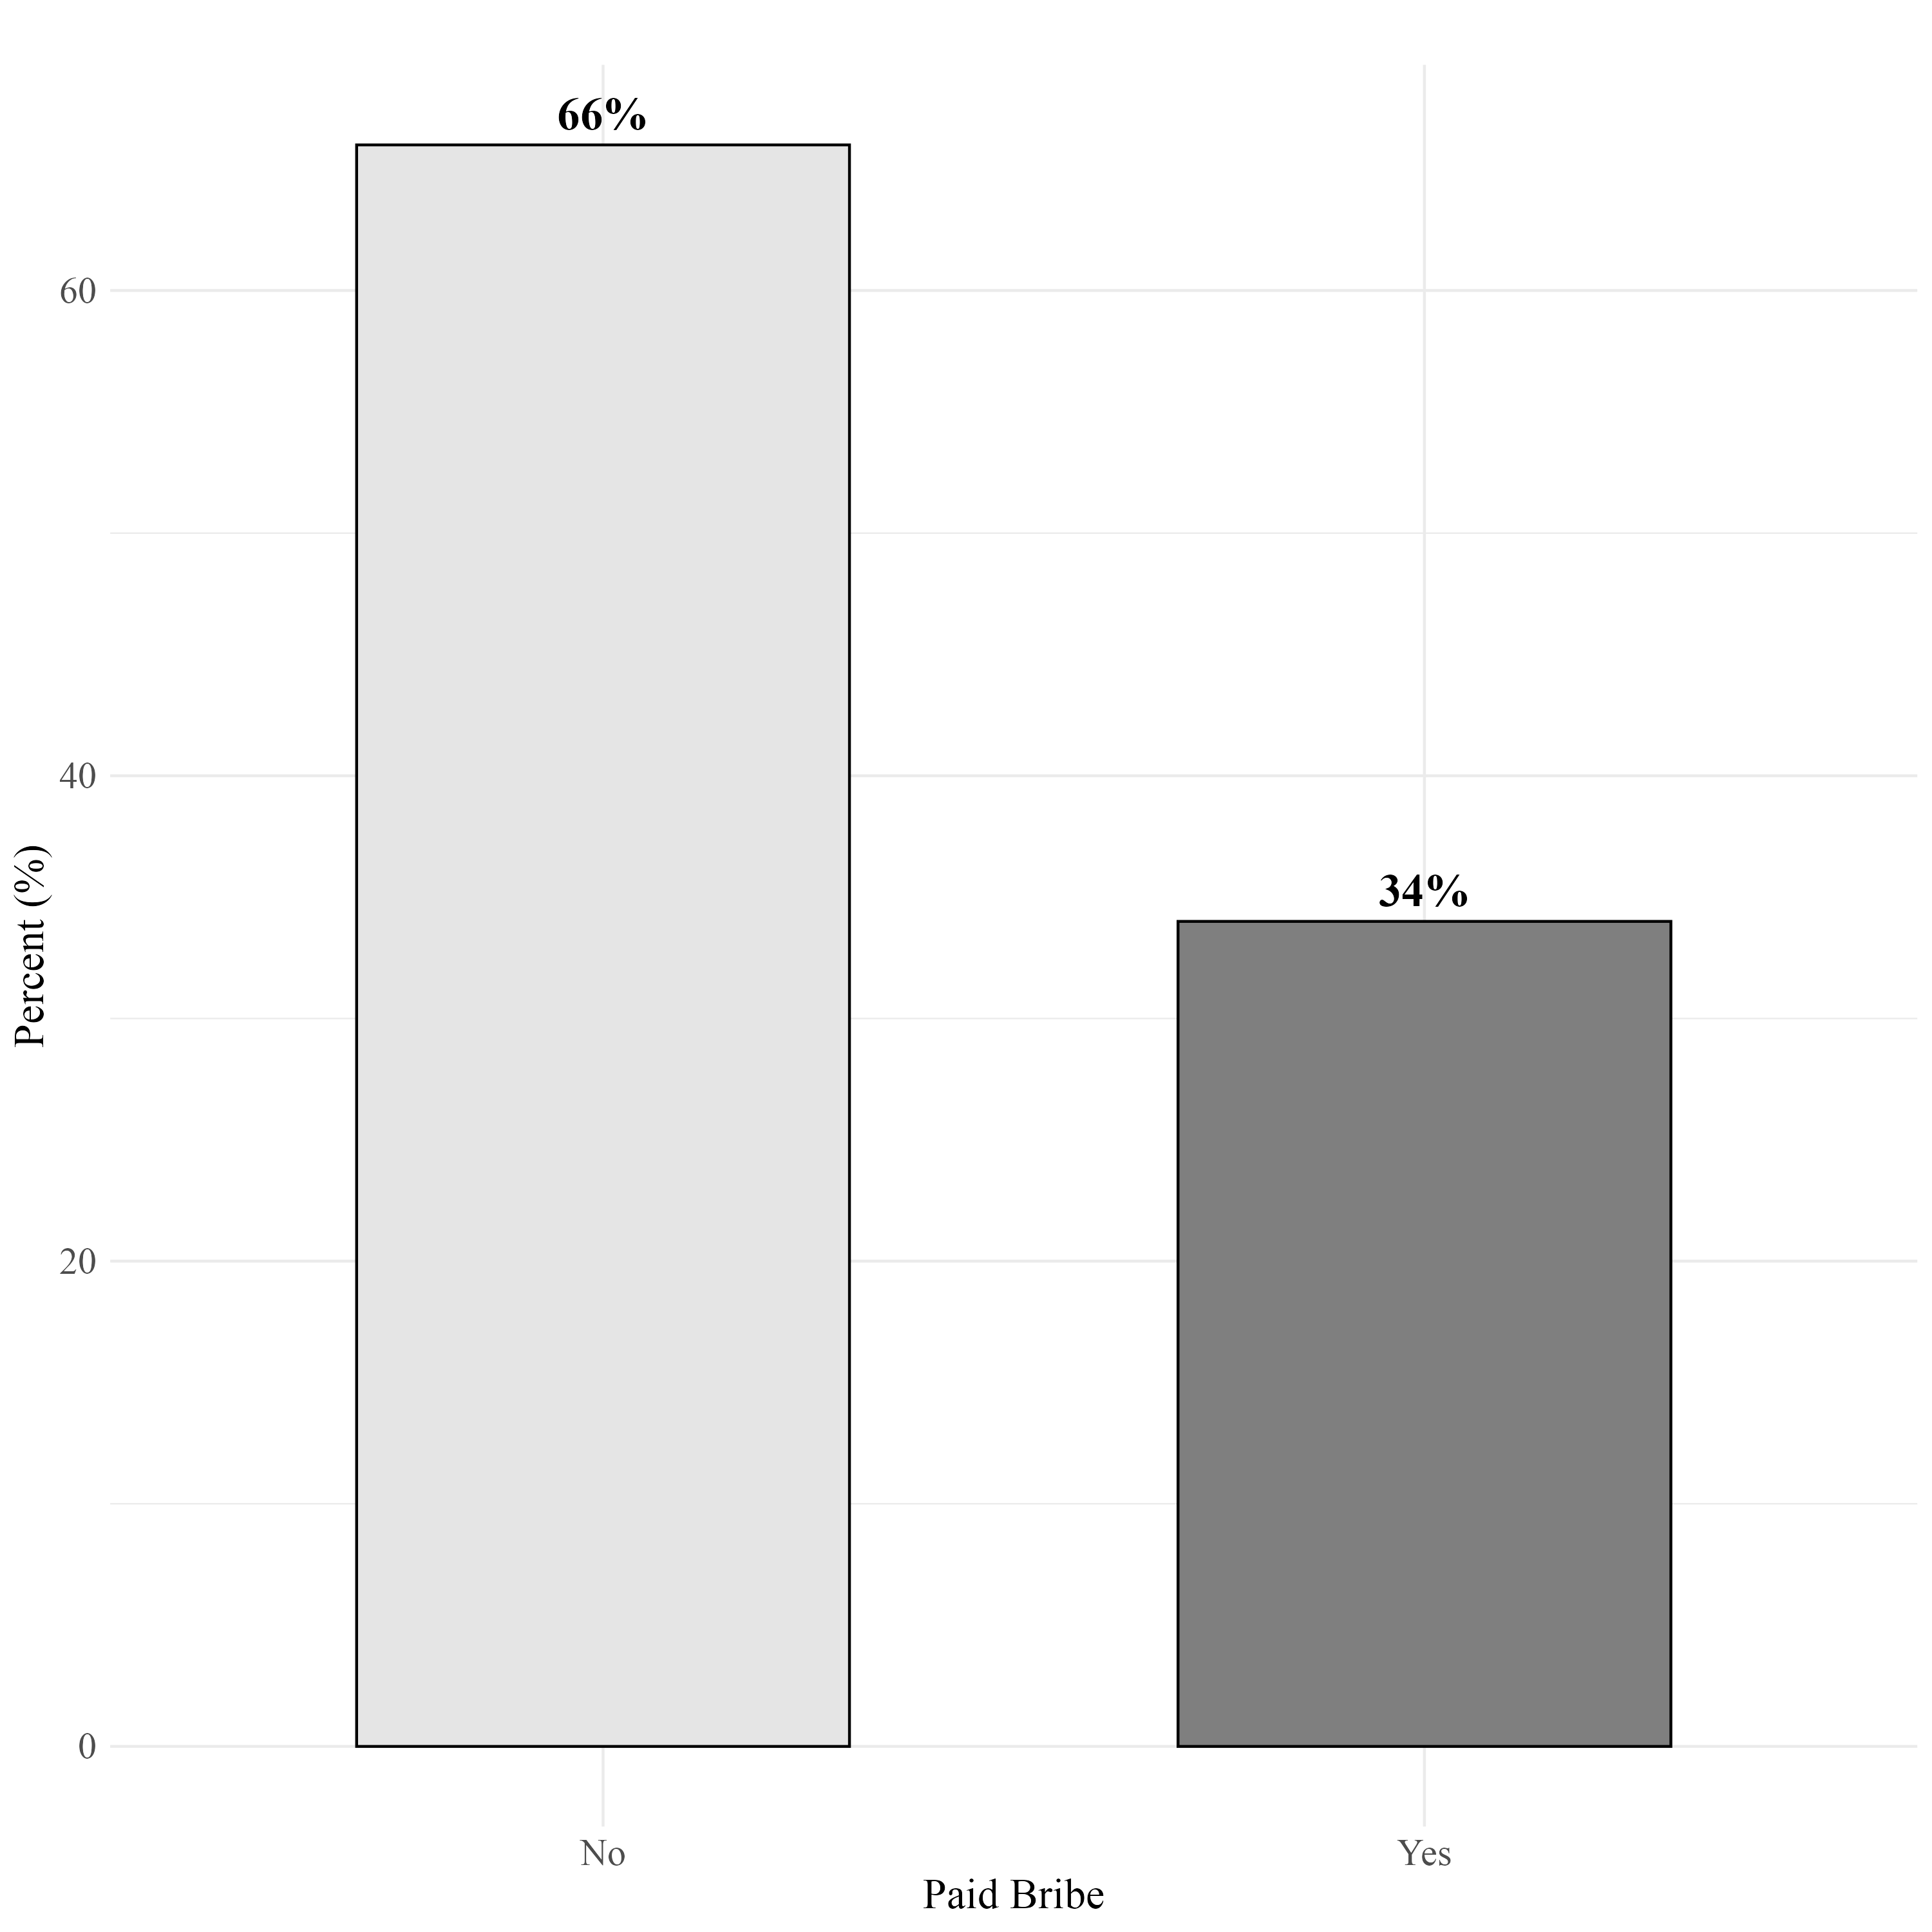
\includegraphics[scale=0.35]{03_graphs/paid_bribe_sch_yr.png}}
\begin{minipage}{0.6\linewidth}
\vspace{3pt}
\footnotesize{\justify\textbf{Notes}: Parents report whether they paid a bribe to get a child a school slot in the last year.}
\end{minipage}
\end{figure}
\end{singlespace}


\end{singlespace}

\clearpage

\singlespacing

%This text contains \charactercount{main} characters.

\printbibliography[title={References}] \pagebreak 
\end{document}


